\documentclass[twocolumn,secnumarabic,amssymb, nobibnotes, aps, prl,
superscriptaddress, nobalancelastpage]{revtex4}
\newcommand{\revtex}{REV\TeX\ }
\newcommand{\classoption}[1]{\texttt{#1}}
\newcommand{\macro}[1]{\texttt{\textbackslash#1}}
\newcommand{\m}[1]{\macro{#1}} \newcommand{\env}[1]{\texttt{#1}}
\setlength{\textheight}{9.5in} \usepackage{graphicx}
\setlength{\belowcaptionskip}{6pt}
\usepackage{amsmath} \usepackage{braket} \usepackage{epsfig}
\usepackage{upgreek}

\newcommand{\tot}{\ensuremath{\sigma_{\text{tot}}}}
\newcommand{\tots}{\ensuremath{\sigma_{\text{tot}}\,}}
\newcommand{\totE}{\ensuremath{\sigma_{\text{tot}}(E)}}
\newcommand{\totEs}{\ensuremath{\sigma_{\text{tot}}(E)\,}}

\newcommand{\gam}{\ensuremath{\gamma} ray}
\newcommand{\gams}{\ensuremath{\gamma} rays}

\begin{document}

\begin{abstract}
    Isotopically-resolved neutron total cross sections of $^{16,18}$O,
    $^{58,64}$Ni, and $^{112,124}$Sn have been measured at the Los Alamos
    Neutron Science Center (LANSCE) at intermediate energies (3-500 MeV) by
    leveraging waveform digitizer technology. The results are in good agreement
    with previous measurements that used analog techniques on natural targets,
    excepting small deviations at high energies, and complete the campaign of
    \tot measurements we initiated with the case study of $^{40,48}$Ca in 2009.
    The \tots relative differences between isotopes (e.g.,
    $\frac{\upsigma_{\text{Ni}^{64}}-\upsigma_{\text{Ni}^{58}}}
    {\upsigma_{\text{Ni}^{64}}+\upsigma_{\text{Ni}^{58}}}$)
    depart from the simple isoscalar picture and reveal additional
    information about the isovector components needed for an
    accurate optical model (OM) description away from stability. Digitizer-enabled 
    \tot-measurement techniques are discussed and a preliminary Dispersive Optical
    Model (DOM) analysis using these data is presented.
\end{abstract}

\title{Isotopically-Resolved Neutron Total Cross Sections From 3-500 MeV}

\author{C.~D.~Pruitt}  \email[Corresponding author:]{cdpruitt@wustl.edu}
\author{R.~J.~Charity}
\author{D. E.~M.~Hoff}  
\author{L.~G.~Sobotka}
\author{K.~W.~Brown} \altaffiliation{Present Address: \textit{National
        Superconducting Cyclotron Laboratory, Departments of Physics and
Astronomy, Michigan State University, East Lansing, MI 48824, USA}}
\author{J.~M.~Elson}
\affiliation{Department of Chemistry, Washington University, St. Louis, MO 63130}

\author{H. Y. Lee}
\author{M. Devlin}
\author{N. Fotiadis}
\author{S. Mosby}
\affiliation{Los Alamos National Lab, Los Alamos, NM 87545, USA}
\maketitle

Neutron scattering is a direct, Coulomb-insensitive tool for probing the nuclear
environment. The simplest measurement of neutron interaction with a nucleus,
the energy-dependent neutron total cross section, \totE, provides fundamental 
information about
nuclear size and the ratio of elastic-to-inelastic components of nucleon
scattering. Additionally, \tots data are sensitive to a variety of nuclear 
properties of great interest including the neutron skin of neutron-rich nuclei
\cite{Mahzoon2017} and thus the density dependence of the symmetry 
energy $L$, essential for an accurate neutron star equation-of-state (EOS)
\cite{Fattoyev2012, Vinas2014, Brown2000}. 

The earliest model for neutron scattering (a ``strongly-absorbing sphere" 
picture) describes the nucleus as a constant-density sphere that interacts strongly with 
incident neutrons approaching within a nuclear radius \cite{Feshbach1949}. In this 
picture devoid of nuclear structure, \totEs depends only
on size scaling of the interacting bodies:
\begin{equation} \label{eq1}
    \sigma_{tot}(E,A) \propto \frac{A^{\frac{2}{3}}}{E}
\end{equation}
where A, A' are the masses of the target isotopes and E is the incident neutron energy 
\cite{Fernbach1949, Satchler1980}. The relative difference between isotopes is thus constant with respect to energy:
\begin{equation}
    \frac{\sigma_{A}-\sigma_{A'}}{\sigma_{A}+\sigma_{A'}} =
    \frac{A^{\frac{2}{3}}-A'^{\frac{2}{3}}}{A^{\frac{2}{3}}+A'^{\frac{2}{3}}}
\end{equation}
While on \textit{average}, experimental \totEs data comport with this naive model,
the main disinguishing feature of \totEs data are the large 
oscillations about the average, clearly visible in Fig. \ref{GlobalTrends} 
\cite{McVoy1967, Satchler1980}.

\begin{figure*}
    \includegraphics[scale=0.3]{figures/globalTrends.png}
    \caption{(Color online) Total neutron cross sections are shown from 2-400
        MeV for several nuclides ranging from A=12 to A=208. Grossly, cross sections
        increase as A$^{\frac{2}{3}}$ due to from simple size scaling and
        decrease as E$^{frac{1}{2}}$ as the neutron wavelength shortens. At higher energy, large oscillations are clearly
        visible as is the trend for their maxima to shift to \textit{higher} energies as
        A is increased. At low
        energies where the density of states is lower (up to a few MeV below the
        neutron separation energy), resonance structures are visible especially
        for light nuclides.}
    \label{GlobalTrends}
\end{figure*}
Early attempts to explain these large oscillations employed a "resonance" model where
an integer number of wavelengths from an incident neutron partial wave fit inside the 
nuclear potential. In this picture, to maintain constant phase of the
oscillations, E must \textit{decrease} as A is increased \cite{Peterson1962, 
Satchler1975}. However, examination of \totEs for many nuclides shows that to
maintain constant phase as nuclear size 
grows, the E must also \textit{increase}:
\begin{equation} \label{eq2}
    \phi(E,A)_{exp} \propto \frac{A^{\frac{1}{3}}}{E^{\frac{1}{2}}}
\end{equation}
Peterson explained this observed phase dependence as a "nuclear Ramsauer effect", the 
result of interference between neutron flux traveling around the nucleus and
through the nucleus analagous to the effect seen for elastic electron scattering
in noble gases \cite{Fernbach1949, Lawson1953, Peterson1962}.
Thus the magnitude of the oscillations indicate that the total cross section has a 
significant elastic component that in turn implies a much larger mean free path of
neutrons through the nucleus than might be otherwise expected \cite{Mohr1955}.

Optical models (OMs) successfully reproduce the general
features of these \tots data across the chart of nuclides up to several hundred
MeV \cite{}. Despite the excellent agreement with experiment, optical model
predictions involve the interaction of many partial waves and are
phenomenologically derived, making intuitive understanding difficult. Thus
several authors have sought to clarify the relative importance of the various components of 
the optical potential (spin-dependence of the nucleon-nucleus force, surface vs. volume, 
etc.) \cite{Gould1986, Anderson1990, Hodgson1967}
Gould et al. that defined a spin-spin cross section $\sigma_{ss}(E)$ \cite{Gould1986}, Anderson and Grimes defined an
isospin-isospin cross section that defined a For highly asymmetric nuclei (in which isovector components of 
the optical potential become increasingly important), their utility diminishes. 
Constraining these
components requires both proton and neutron scattering data for a
given nucleus across a wide energy range \cite{DOMPaper}.
The experimental difficulty of neutron scattering measurements has meant that these 
data are often limited or missing entirely despite their value for extending OM 
analyses toward the driplines.

\section{Experimental Considerations}
By scattering secondary radioactive beams off of hydrogen targets in inverse
kinematics, proton-scattering experiments are possible even on highly unstable
nuclides. In contrast, because neutrons themselves must
be generated as a secondary radioactive beam, neutron-scattering experiments are 
restricted to normal kinematics and \tots measurements are possible only for 
relatively stable nuclides that can be formed into a target. At present, 
\tots measurements above the resonance region on nuclides with half-lives shorter than
the timescale of days are technically infeasible, though a handful have been carried 
out on samples with half-lives in the tens to thousands of years
\cite{TritiumMeasurement, Tc99Measurement, U233Measurement}. 

Traditionally, \tots measurements have relied on analog techniques for
recording events, techniques that suffer from a large per-event deadtime of
up to several $\mu$seconds. Thus for a typical intermediate-energy \tots measurement 
with dozens or hundreds
of energy bins, achieving statistical uncertainty at the level of 1\% requires a 
sample in the tens of grams \cite{Finlay1993, Abfalterer2001}. Producing an 
isotopically-enriched sample of this size is often prohibitively 
expensive. Indeed, a literature search for isotopically-resolved \tots measurements
reveals a paucity of data from 1-300 MeV, even for closed-shell isotopes of special 
importance like $^{3,4}$He, $^{64}$Ni, $^{204}$Pb (see Table \ref{IsotopeTable}).

\begin{table}[ht]
    \caption{Intermediate-energy $\sigma_{tot}$ data at closed shells in Z from
    EXFOR Database}
    \label{IsotopeTable}
    \begin{center}
        \begin{tabular}{ c c c c }
            \hline
            Isotope & Natural Abundance & Energy Range (MeV) & Reference\\
            \hline

            $^{3}$He & $2\times 10^{-4}\%$ & $1.5 - 40$ & \cite{Haesner1983}\\
            $^{4}$He & $>99.9\%$ & $0.7-30$ & \cite{Goulding1973}\\
            & & $2-40$ & \cite{Haesner1983}\\
            & & $77-151$ & \cite{Measday1966}\\

            $^{16}$O & $99.8\%$ & $0.2-49$ & \cite{Perey1972}\\
            & & $5-600$ & \cite{Finlay1993}\\

            $^{18}$O & $0.20\%$ & $0.1-2.5$ & \cite{Vaughn1965}\\
            & & $2.5-19$ & \cite{Salisbury1965}\\

            $^{40}$Ca & $96.9\%$ & $<0.1-6.4$ & \cite{Johnson1973}\\
            & & $5.3-560$ & \cite{Abfalterer2001}\\

            $^{48}$Ca & $0.187\%$ & $0.6-5.2$ & \cite{Harvey1985}\\
            & & $12-276$ & \cite{Shane2010}\\

            $^{58}$Ni & $68.1\%$ & $<0.1-68$ & \cite{Perey1993,
        Perey1993TechReport, Perey1993ENDF}\\

            $^{64}$Ni & $0.926\%$ & $14.1$ & \cite{Dukarevich1967}\\

            $^{112}$Sn & $0.97\%$ & $<0.1-1.4$ & \cite{Timokhov1989}\\
            & & $14.1$ & \cite{Dukarevich1967}\\

            $^{124}$Sn & $5.79\%$ & $0.3-5.0$ & \cite{Harper1982}\\
            & & $5.1-26$ & \cite{Rapaport1980, Mirzaa1978}\\

            $^{204}$Pb & $1.4\%$ & $<0.1-27$ & \cite{Carlton2003}\\

            $^{208}$Pb & $52.4\%$ & $<0.1 - 695$ & \cite{Harvey1999}\\
            & & $5-600$ & \cite{Finlay1993}\\

            \hline
        \end{tabular}
    \end{center}
\end{table}

Recently developments in waveform digitizer technology, however, have made it
possible to reduce the per-event deadtime by an order of magnitude or more,
enabling a corresponding reduction in the sample size needed. Thus in 2008 we
embarked on a campaign of \tots measurements
on isotopically-enriched samples, starting with a case study on $^{40,48}$Ca
from 15-300 MeV \cite{Shane2010}. The data from this measurement have been 
incorporated into a 
comprehensive Dispersive Optical Model (DOM) analysis \cite{DOMPapers} yielding 
proton and neutron spectroscopic factors, charge radii, and neutron
skins for these nuclei \cite{NeutronSkinCa48}. We now present \tots results for
the important closed-shell nuclides $^{16,18}$O, $^{58,64}$Ni, and
$^{112,124}$Sn and describe further developments in the digitizer-mediated
approach.

\section{Experimental Details}
All neutron total cross section measurements were carried out at the 15R
beamline at the Weapons Neutron Research (WNR) facility of the Los Alamos
Neutron Science Center (LANSCE) during two run cycles (November 2016 and
September 2017). Our experiment was modeled on previous \tots measurements at WNR
\cite{Finlay1993,Abfalterer2001,Shane2010}. At WNR, broad-spectrum 
neutrons up
to 800 MeV are generated by impinging proton pulses onto a water-cooled, 7.5
cm-long tungsten target (see Fig. \ref{ExperimentalApparatus}). Before the beam
enters the experimental area, a
permanent magnet deflects all charged particles generated by the proton pulses, 
allowing only neutrons and gamma rays to reach the flight path. At the
entrance to the flight path, the beam was collimated to 0.200" using steel
donuts with a total thickness of 24" inches and hardened using a plug of Hevimet (90\% W, 6\% Ni, 4\% Cu by weight) 
inserted at the upstream entrance of the
collimation stack. After collimation, the beam passed through a flux 
monitor, the sample of interest held in a sample changer, a veto detector, and finally
the time-of-flight (TOF) detector approximately 25 meters from the neutron
source. The veto paddle allowed for rejection of any charged particles created
by the neutron beam in-flight after the permanent magnet.
All detectors consisted of BC-400 fast-scintillating plastic mated with 
photomultiplier tubes (PMTs) and encased in a plastic or
aluminium structural housing. Signals from all detectors and
the target changer were relayed to a 500-MHz CAEN DT-5730 waveform digitizer
running custom software, described later in the analysis section.

The particular neutron beam structure at WNR dictates the energy range
achievable for \tots measurements (see Fig. \ref{BeamStructure}).
At the largest timescales, proton pulse trains 625 $\mu$seconds long,
called ``macropulses", are delivered to the tungsten target at 120 Hz. Each 
macropulse
consists of ~350 individual proton pulses, called ``micropulses", themselves
spaced 1.8 $\mu$seconds apart. Each micropulse consists of a single proton 
packet $<$1 ns wide when 
it arrives at the
tungsten target that generates gamma rays and neutrons within a tight
temporal-spatial range. As neutrons from a single micropulse travel along the 
beam path, high-energy neutrons separate in time from lower-energy neutrons so 
that neutron energy can be determined by standard TOF techniques (see
\cite{TOFTechniques} for details). Because the $\gamma$ rays and high-energy
neutrons from later pulses can catch up to slower neutrons from an earlier
micropulse, the distance of the TOF detector determines both the minimum 
neutron energy that can be unambiguously detected
and also the maximum instantaneous event rate, critical to correcting for
per-event deadtime.

\begin{figure}
    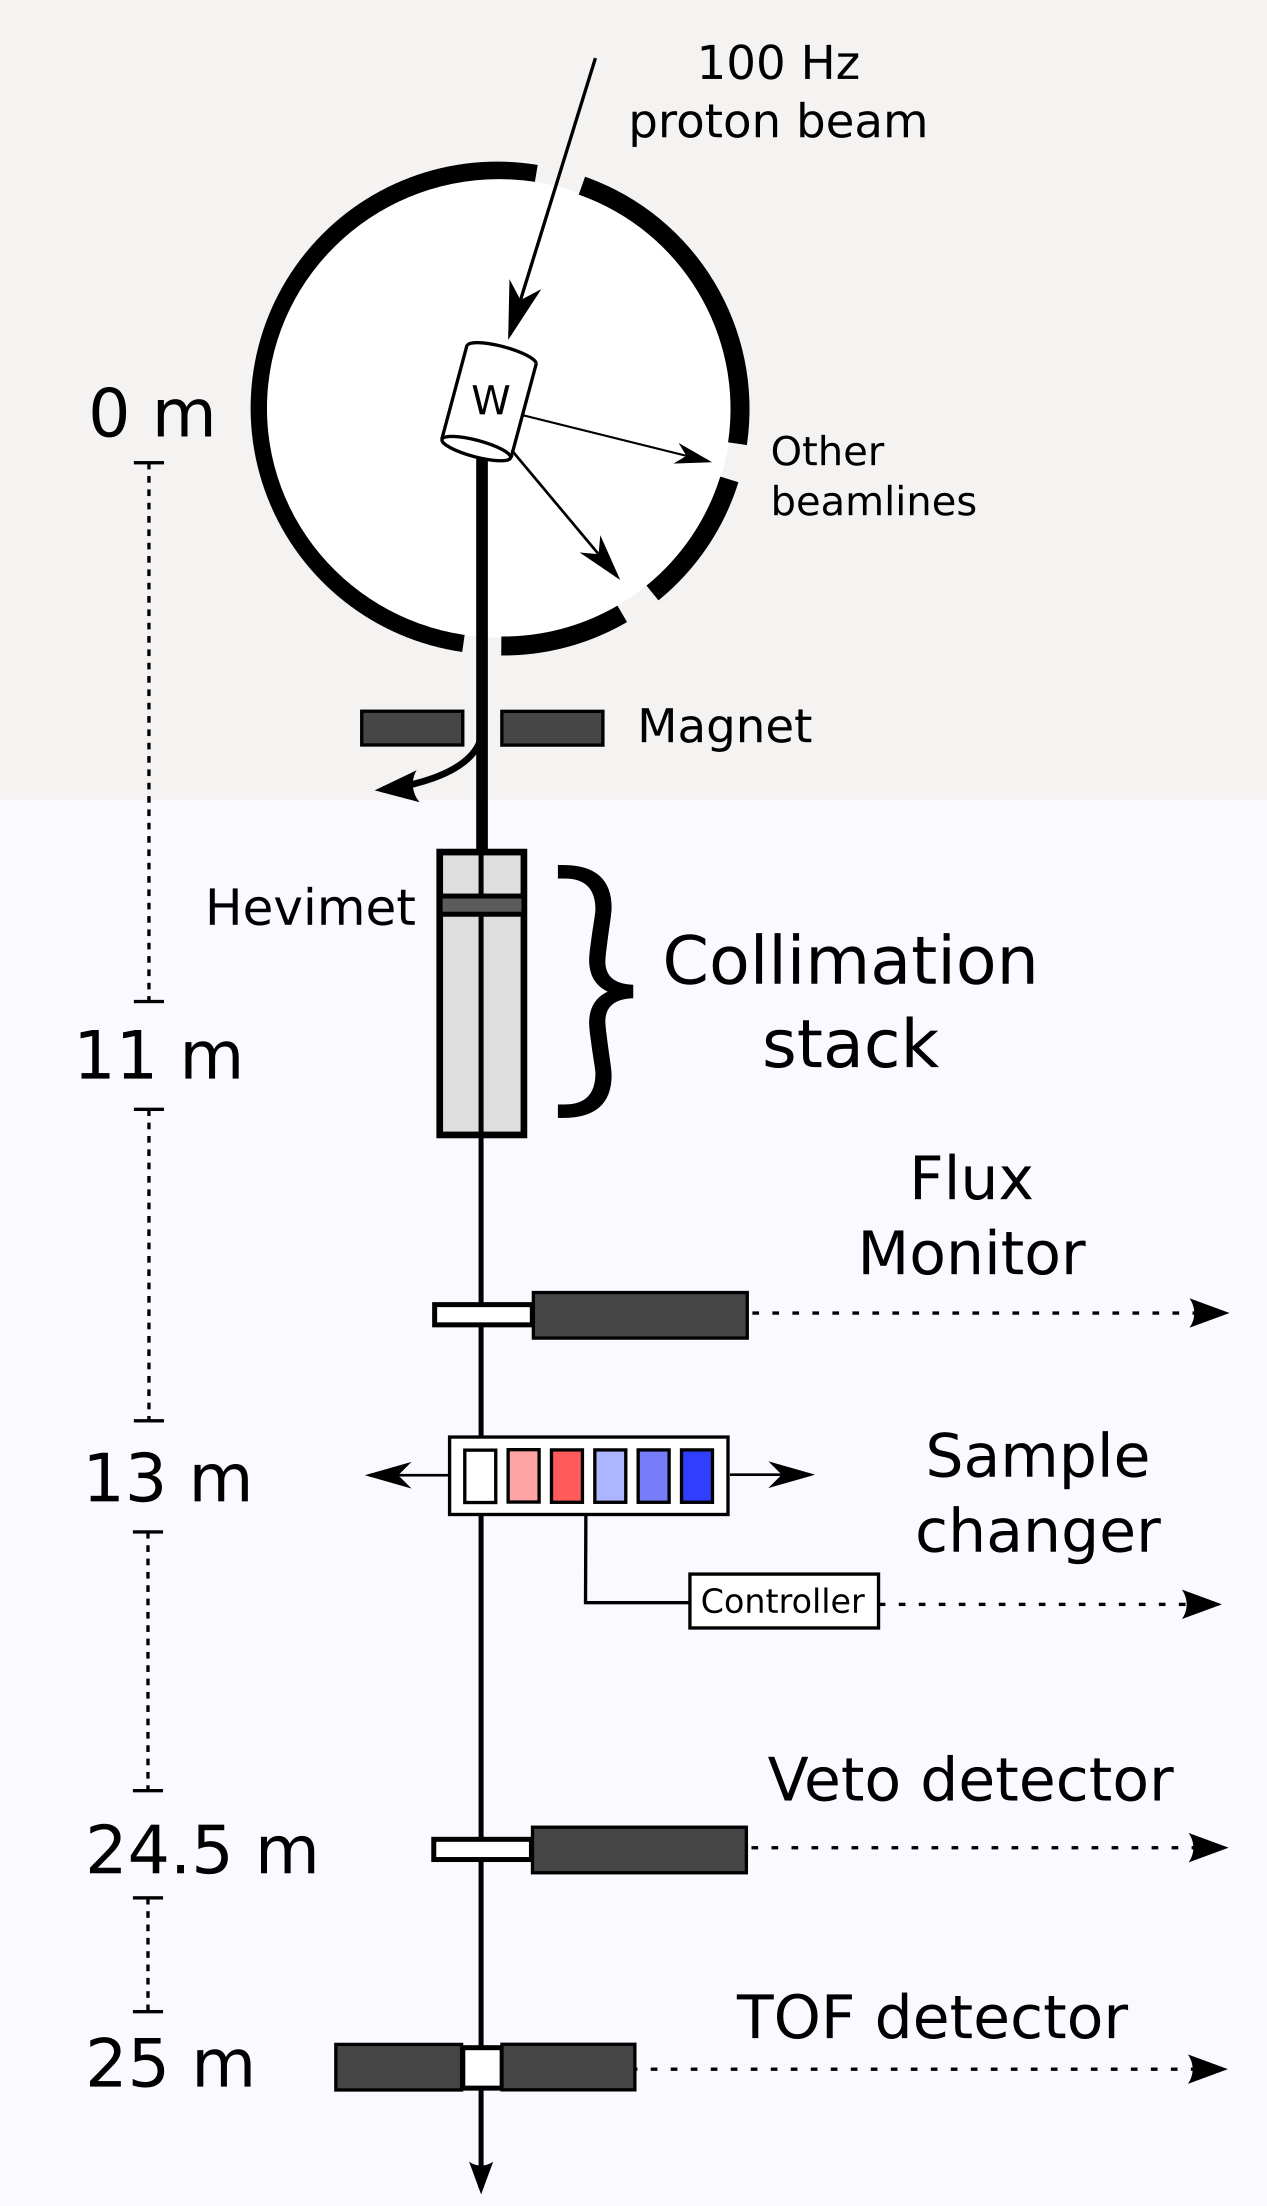
\includegraphics[scale=0.7]{figures/ExperimentalSetup.png}
    \caption{(Color online) Experimental configuration at WNR facility. The
    neutron beam passes through a collimation stack where it is collimated to
    0.2" en route to the detectors used in the experiment. Targets are cycled
    in-beam using a linear actuator with a period of 150 seconds.
    Times-of-flight are detected by the main detector and used to calculate 
    neutron energies.}
    \label{ExperimentalApparatus}
\end{figure}

\begin{figure*}
    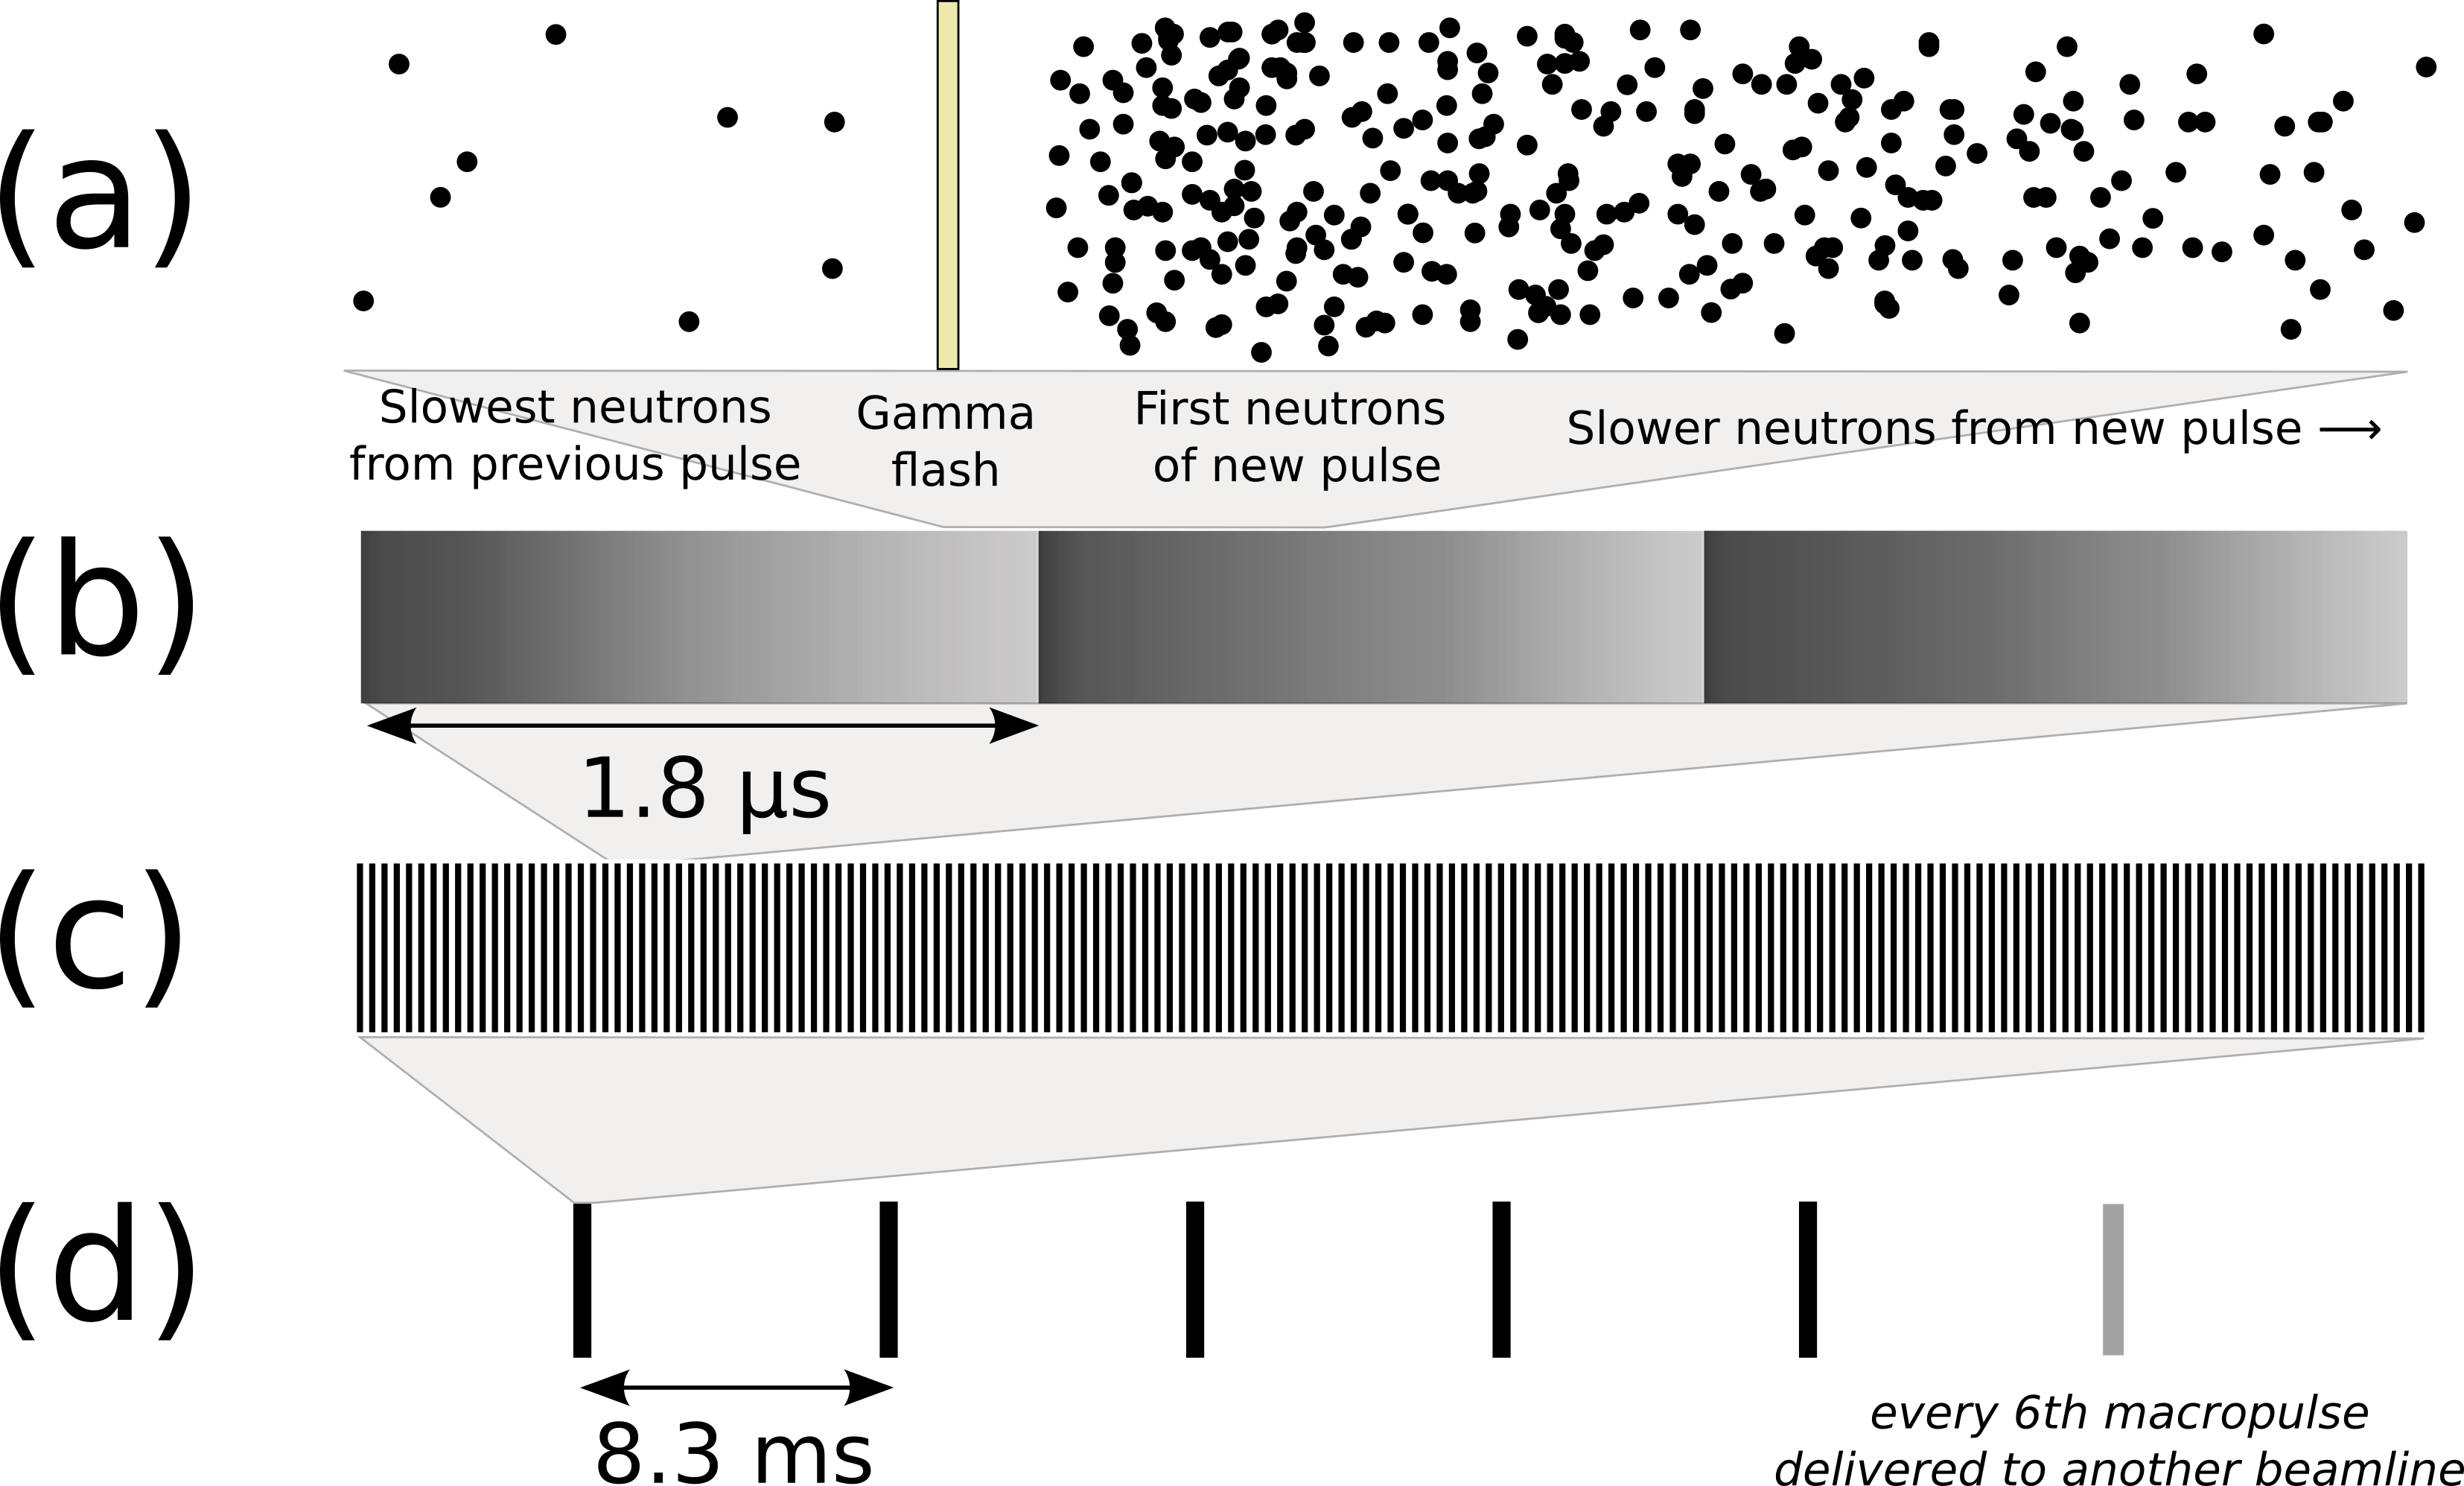
\includegraphics[scale=0.4]{figures/beamStructure.png}
    \caption{(Color online) Neutron beam structure at WNR facility.
        ``Macropulses" of protons (bottom row on figure) are delivered to Target 
        4, where they generate
        neutrons by spallation on a tungsten target. Each macropulse consists of
        $\approx$ 350 proton ``micropulses" (second from bottom row). Neutrons
        from each micropulse (second from top row) disperse in
time as they travel along the flight path so that $\gamma$ rays and high-energy 
neutrons catch up
to low-energy ones from the previous pulse.}
    \label{BeamStructure}
\end{figure*}

A programmable sample changer with six positions
was used to cycle each sample into the beam at a regular interval of 150 seconds 
per sample. An analog signal from the sample changer to indicate the current
position was recorded once per macropulse. Variations in beam flux 
between macropulses were monitored by the flux monitor detector. To account for 
charged-particle production in the 
samples and in air along the flight path, a veto paddle was installed immediately
upstream of the TOF detector.

All detector and sample signals were recorded by a 500 MHz, 8-
channel CAEN DT5730 waveform digitizer. Custom software was used to run the 
digitizer in two complementary modes, referred to as ``DPP mode" and ``waveform 
mode". In DPP mode, triggers are generated by the digitizer's onboard peak-
sensing firmware. For each trigger, a set of data was recorded: the trigger 
timestamp, two charge integrals over the peak, with the integral boundaries 
specifiable by the experimenter, and a small piece of the raw digitized signal
, referred to as a ``wavelet". DPP mode was used for the vast majority of the 
experiment and accounts for $\approx$99\% of the total data volume. In waveform mode, 
the digitizer performs no peak-sensing and was externally triggered. Upon 
triggering, the trigger timestamp and a very long wavelet (60 microseconds) 
were recorded. While waveform mode data accounts for only ~1
\% of the total data, the instantaneous data rate is much higher than in DPP 
mode because hundreds of microseconds of consecutive waveform samples are 
stored. Roughly once every three seconds, the digitizer was switched to 
waveform mode for one macropulse, then immediately switched back to DPP mode.  

Except for the oxygen isotopes and rhodium sample, all samples were prepared as 
right cylinders 
$\approx$8.25 mm in diameter and ranging from 10-27 mm in length (see Table
\ref{SampleTable}). In addition
to isotopically-enriched samples, a natural-abundance sample was prepared for 
each element under study. Each of these samples was inserted into a styrofoam
sleeve seated in the sample changer. This design minimizes the amount of non-target
mass proximate to the neutron beam path.
The oxygen isotopes were prepared as water samples to increase the areal density 
of atoms and for ease of handling. Each water sample was contained by a
cylindrical brass vessel with very thin (0.002") brass endcaps, minimizing beam 
attenuation in the vessel. Calculating oxygen cross sections
required subtracting the well-known hydrogen
cross section (available in the literature) from the raw H$_{2}$O result. 
Because of the additional
uncertainty inherent to this kind of subtractive measurement, a D$_{2}^{nat}$O
sample was also prepared from which the literature D$_{2}$ \tots could be
subtracted to recover the oxygen \tot, as an additional cross-check.
Due to its poor machining properties, the rhodium sample was prepared by
stacking a series of thin rhodium discs rather than by producing a fused 
cylinder. These discs were contained by a cylindrical plastic case with open
ends, similar to the styrofoam sleeves.

\begin{figure}
    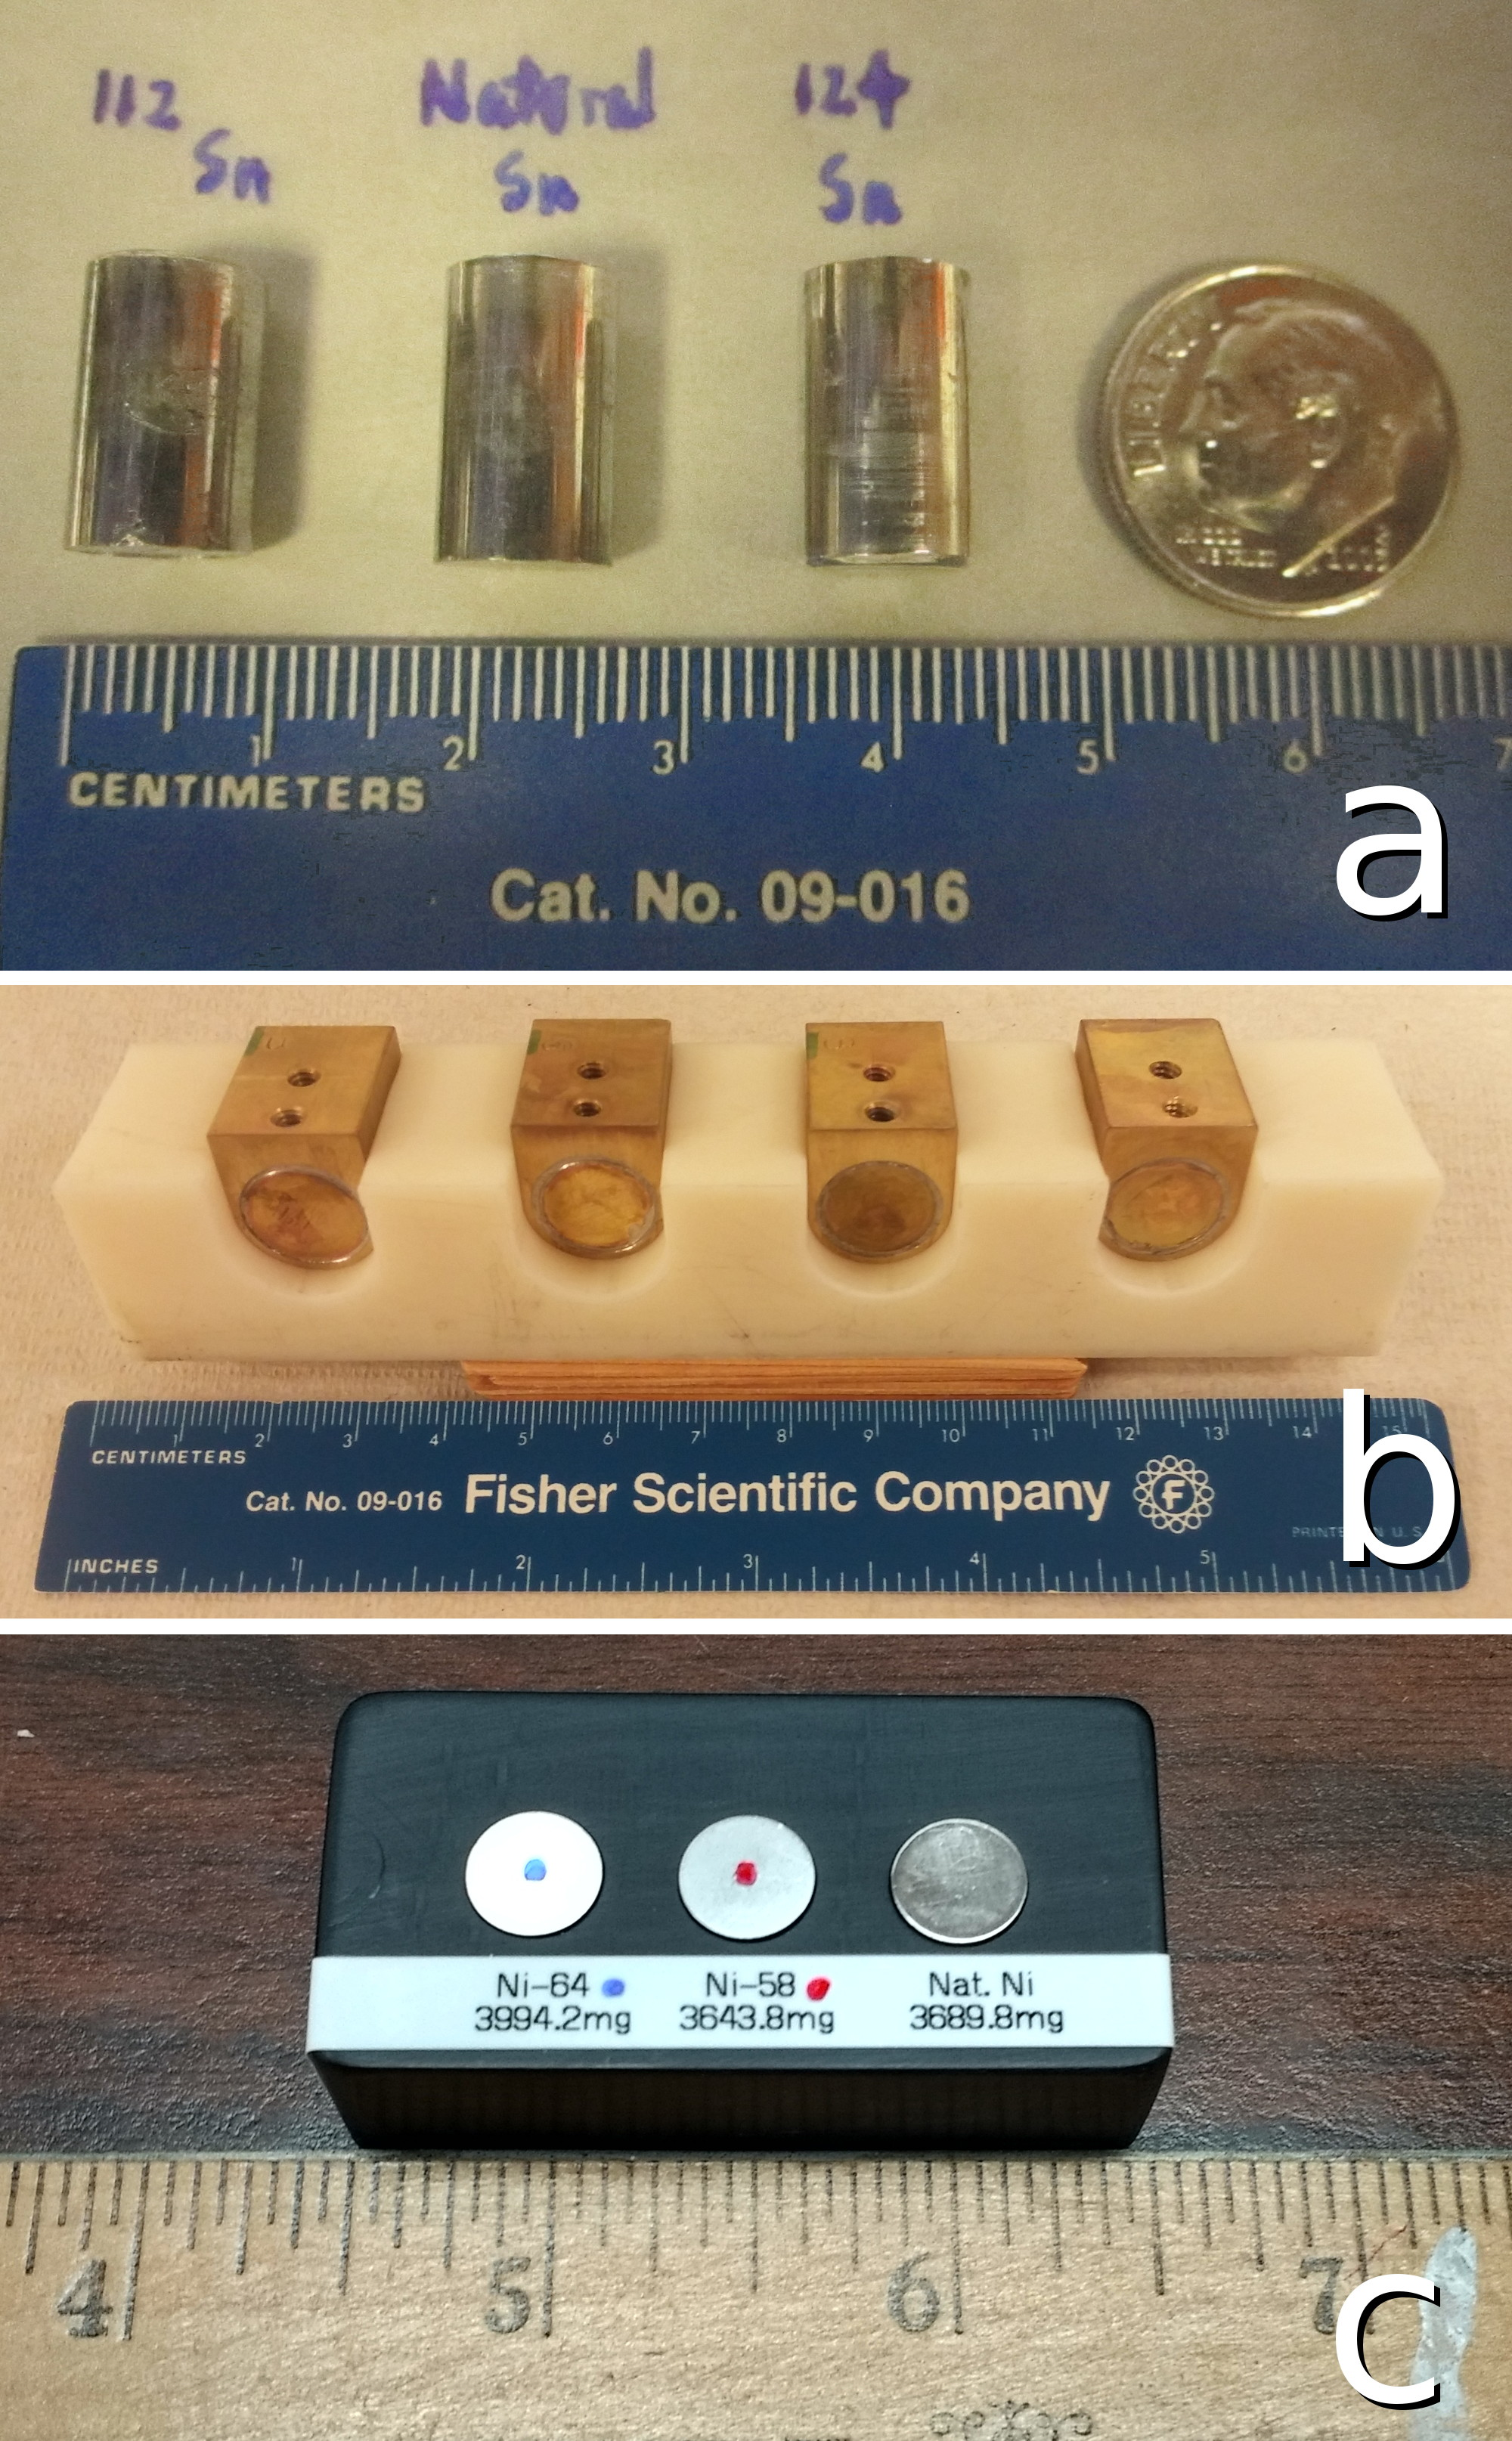
\includegraphics[scale=0.23]{figures/AllIsotopicSamples.jpg}
    \caption{(Color online) Section a shows the ${^{112,nat,124}}$Sn samples used in
        the \tots measurement. Section b shows the target vessels used to hold
        water samples for the ${^{nat, 18}}$O \tots measurement. Section c shows
    ${^{58,nat,64}}$Ni samples used in the \tots measurement.}
    \label{SamplesImage}
\end{figure}

\begin{table*}[t]
    \caption{Sample Characteristics}
    \label{SampleTable}
    \begin{center}
        \begin{tabular}{ c c c c c c }
            \hline
            Isotope & Nat. Abundance & Length [mm] & Diameter
            [mm] & Mass [g] & Isotopic Purity\\
            \hline

            $^{nat}$C & - & 13.66$\pm$0.02 & 8.26$\pm$0.005 & 1.2363 & -\\
            $^{nat}$C & - & 27.29$\pm$0.02 & 8.26$\pm$0.005 & 2.4680 & -\\

            H$_{2}^{nat}$O & - & 20.0 & 10.0 & N/A & - \\
            D$_{2}^{nat}$O & - & 20.0 & 10.0 & N/A & - \\
            H$_{2}^{18}$O & $0.20\%$ & 20.0 & 10.0 & N/A & $99\%$\\

            $^{58}$Ni & $68.077\%$ & 7.97$\pm$0.03 & 8.18$\pm$0.02 & 3.6438 & $99.6\%$\\
            $^{nat}$Ni & - & 8.00$\pm$0.03 & 8.20$\pm$0.02 & 3.6898 & -\\
            $^{64}$Ni & $0.926\%$ & 7.96$\pm$0.02 & 8.20$\pm$0.04 & 3.9942 & $92.2\%$\\

            $^{103}$Rh & $100\%$ & ?$\pm$? & ?$\pm$? & 2.8359 & $99.9\%$\\

            $^{112}$Sn & $0.97\%$ & 13.65$\pm$0.03 & 8.245$\pm$0.005 & 4.9720 & $99.9\%$\\
            $^{nat}$Sn & - & 13.68$\pm$0.03 & 8.245$\pm$0.005 & 5.3263 & -\\
            $^{124}$Sn & $5.79\%$ & 13.73$\pm$0.03 & 8.245$\pm$0.005 & 5.5492 &
            $99.9\%$\\

            $^{nat}$Pb & - & 10.07$\pm$0.02 & 8.27$\pm$0.01 & 6.130 & -\\

            \hline
        \end{tabular}
    \end{center}
\end{table*}

The sample configuration for each run varied, but generally all six positions
on the sample changer were used. For the solid targets, a typical configuration 
was to place an empty styrofoam sample sleeve in the first position as the ``blank", 
$^{nat}$C and $^{nat}$Pb samples in the second and third positions, and the samples of 
interest (e.g., $^{58}$Ni, $^{nat}$Ni, $^{64}$Ni) in the fourth, fifth, and sixth
positions. For water samples, an empty brass vessel was placed in the first
position to serve as the blank.

\section{Experimental Analysis}

The fundamental quantity of interest, \tot, is related to the flux
loss through a sample by:
$$
I_{t} = I_{0}e^{-{\ell\rho\sigma_{tot}}}
$$

or, equivalently,

$$
\tot = -\frac{1}{\ell\rho}
ln \left(\frac{I_{t}}{I_{0}}\right)
$$
where $I_{0}$ is the neutron flux entering the sample, 
$I_{t}$ is the neutron flux transmitted through the sample without interacting,
$\rho$ is the number density of nuclei in the sample, and
$\ell$ is the sample length. Thus for thin or low-density samples, flux 
attenuation through the sample will be very small and large statistics
will be required to determine the cross section to high precision.

To calculate cross sections from the raw event data, a series of corrections
are required. First, all detector events were assigned to their
macropulse and time offsets (accounting for cable and electronics
delay) were applied, synchronizing all detectors with the facility clock. The 
digitized waveform for each event was passed through an offline software CFD logic, 
improving the timing resolution for each event to below 1 ns [insert FWHM from
left/right detectors here].

To improve the macropulse start time resolution (the "starting gun" for
measuring TOF), the \gams were employed. For each macropulse,
all \gams were identified and their average TOF
calculated. The difference between this time and the expected TOF from the TOF
detector distance was applied to all events in that macropulse (see
Fig. \ref{GammaTimeCorrection}). The final time resolution (FWHM of the \gams)
ranged from 0.6-0.8 ns for the O, Ni, Sn, and Rh experiments. This translates to
an energy resolution of 

Because events are not processed instantaneously, there is a brief period,
referred to as the ``deadtime", after each event trigger during which the digitizer
is busy processing that trigger. Any newly-arriving events in this period will be
ignored, privileging events arriving earlier and thus distorting the cross
sections. To remedy this, a rate-dependent deadtime correction for each target must be 
calculated and applied according to standard techniques \cite{Moore1980}.
While deadtime correction schemes that incorporate the possibility of varying
beam flux have been developed
\cite{Moore1980}, we found that, given the deadtimes present in our
experiment, the effect of flux variation on deadtime correction was negligible.
Thus to simplify the correction model, we assumed no variation in beam flux. 
With no beam profile changes between micropulses, the fraction of time $F_{i}$ that 
the digitizer is dead for a given time bin $i$ can be calulated: 

$$
F_{i} = \sum_{j=0}^{N-1} R((i-j)\mod N) \times P(j)
$$
where $N$ is the number of time bins in the micropulse, $R(i)$ is the
rate of events per micropulse in bin $i$, and $P(j)$ is the probability that
the digitizer is still busy from a trigger $j$ bins ago.
To model $P(j)$, we employed a logistic function and fitted it to the observed
spectrum for time differences between adjacent events (see Fig.
\ref{TimeDifferenceBetweenEvents}), in effect allowing for a varying
rather than a fixed deadtime.
The fraction dead $F_{i}$ is in essence a discrete convolution of the TOF spectrum 
with $P(j)$ that allows the deadtime to "wrap around" between adjacent micropulses. 
Typical values for $F_{i}$ in our experiment are shown in Fig.
\ref{DeadtimePlot}. Because trigger processing is done quickly in firmware onboard the
digitizer, the per-event deadtimes affecting our measurement ranged from 150-230
ns, several times smaller than the 1-3 $\mu$s common in previous analog
experiments \cite{Finlay1993, Abfalterer2001}.

Once the fraction dead was identified for each time bin, the number of events
\textit{measured} in a given bin, $E_{m}(i)$, was corrected to the \textit{true} number
of events arriving at the detector in a given bin, $E_{c}(i)$:

$$
E_{c}(i) = -ln\left(\frac{1-\frac{E_{m}(i)}{M}}{(1-F_{i})\times M}\right)
$$
where $M$ is the total number of micropulse periods over which data was taken for a
given target. The difference between the uncorrected and corrected TOF spectra 
is shown in Figure \ref{DeadtimeCorrectedSpectra}. At low energies, the
correction is as low as a few percent, but at high energies, particularly above
70 MeV, the correction is quite significant [insert \% value here].

[More here with a comparison between Bec's and Abfalterer/Finlay's approach to
the same issues].

During analysis, it was noted that occasionally (\~1 in 400 macropulses), one or two 
adjacent macropulses would have an abnormally small number of flux monitor events or 
TOF events. The frequency of these "data dropouts" was similar to the rate of
switching between DPP and waveform modes and we suspect it is related to edge
case behavior right before or after a mode switch. To mitigate this issue,
any macropulse that had less than 50\% of the average event rate in either the
flux monitor or TOF detector channel was ignored during cross section calculation.

After the above corrections, the charged-particle veto was applied. 

[more description here about gamma ray timing precision and a comparison to
that from Bec's experiment].

\begin{figure}
    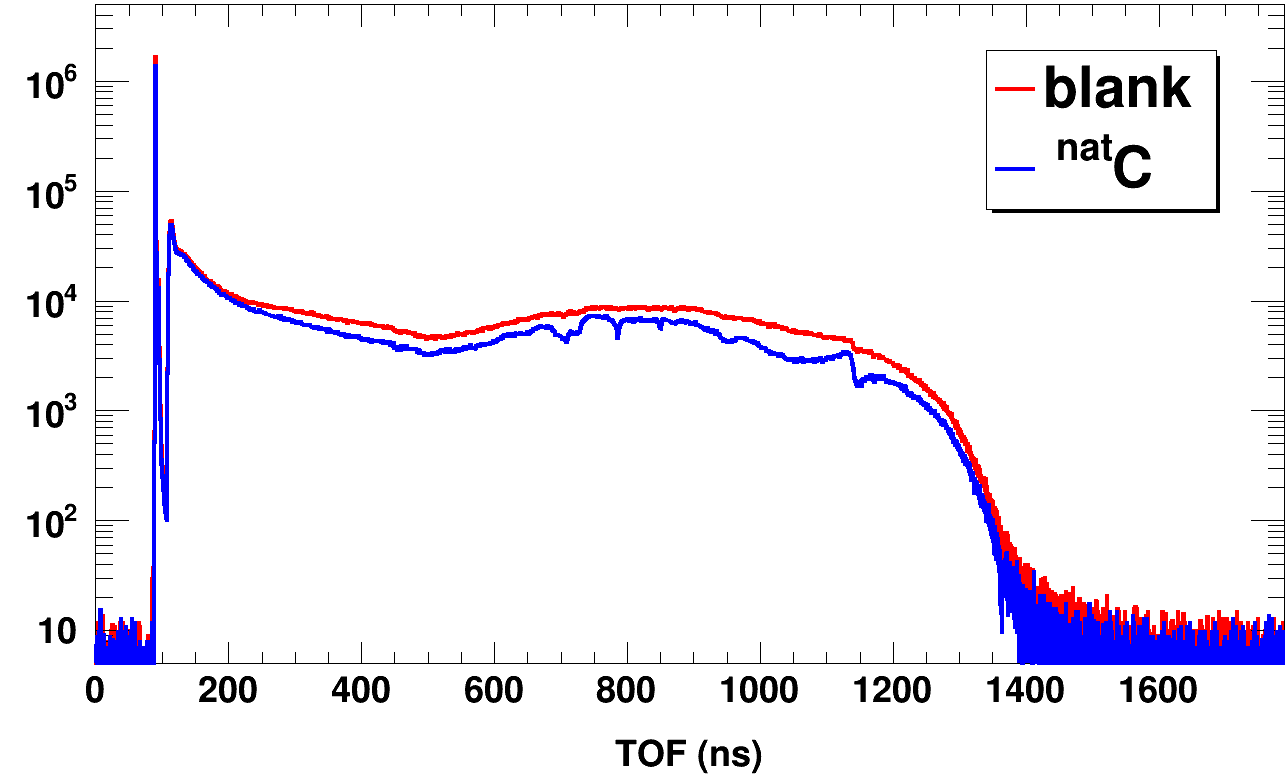
\includegraphics[scale=0.24]{figures/exampleTOFSpectrum.png}
    \caption{(Color online) A typical TOF spectrum is shown for the blank sample (in
        red) and for the $^{nat}$C sample (in blue). Events caused by accelerator 
        ``dark current" are visible as 
    }
\end{figure}

\begin{figure}
    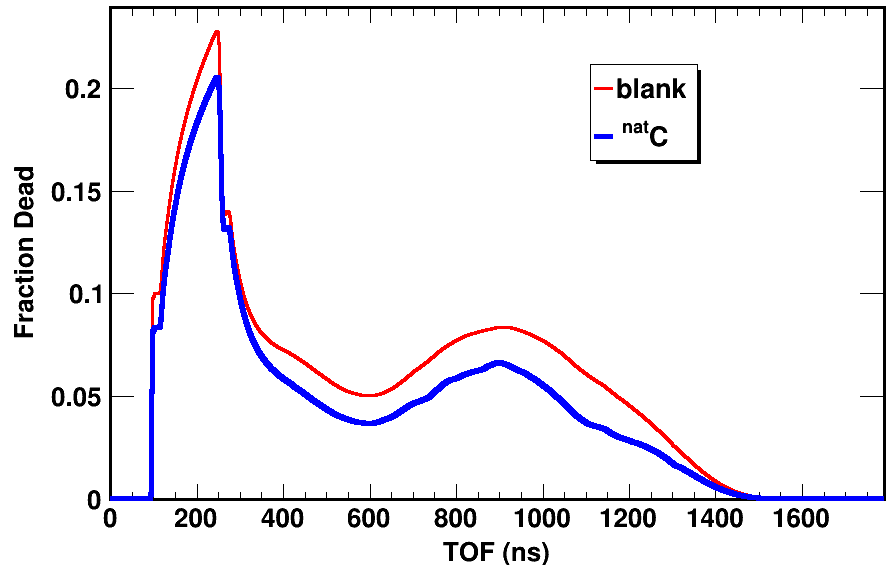
\includegraphics[scale=0.24]{figures/exampleDeadtimeSpectrum.png}
    \caption{(Color online) A typical per-event deadtime spectrum is shown for the 
        blank sample (in red) and for the $^{nat}$C sample (in blue). Only
        high-energy neutrons experience a per-event deadtime $>10\%$.
    }
    \label{DeadtimePlot}
\end{figure}

[describe veto procedure, charge gating procedure, and conversion of TOF to
energy bins]

\section{Error Analysis}

[describe error propagation...? Or this more appropriate for analysis section?]

\section{Experimental Results}

[all cross section plot results]

\section{Discussion}

[Discussion]

\section{DOM Analysis}

[Preliminary DOM Analysis for oxygen]

\section{Conclusion}

[Conclusion]

\section{Acknowledgements}

\begin{figure*}
    \includegraphics[scale=0.35]{figures/FourPanelO.png}
    \caption{(Color online) Neutron total cross sections for $^{16,18}$O.
     Panel one shows our measurement (in red) and literature data from
     Abfalterer (in
     black), where the $^{18}$O values have been shifted up by 1 barn for
     readability. Panel two shows the relative difference between our 
     measurement and the literature data from the first panel. Panels three and
     four show the corresponding absolute and relative cross sections after a
     Pb-C correction, derived from literature data and our Sn dataset,
     are applied.
    }
\end{figure*}

\begin{figure*}
    \includegraphics[scale=0.35]{figures/FourPanelNi.png}
    \caption{(Color online) Neutron total cross sections for $^{58,64}$Ni.
     Panel one shows our measurement (in red) and literature data from
     Abfalterer (in % black).
     Panel two shows the relative difference between our 
     measurement and the literature data from the first panel. Panels three and
     four show the corresponding absolute and relative cross sections after a
     Pb-C correction, derived from literature data and detailed in the text,
     are applied.
    }
\end{figure*}

\begin{figure*}
    \includegraphics[scale=0.35]{figures/FourPanelSn.png}
    \caption{(Color online) Neutron total cross sections for $^{112,124}$Sn.
     Panel one shows our measurement (in red) and literature data from
     Finlay (in % black).
     Panel two shows the relative difference between our 
     measurement and the literature data from the first panel. Panels three and
     four show the corresponding absolute and relative cross sections after a
     Pb-C correction, derived from literature data and detailed in the text,
     are applied.
    }
\end{figure*}

\begin{figure*}
    \includegraphics[scale=0.35]{figures/FourPanelNiIsotopes.png}
    \caption{(Color online) Neutron total cross sections for $^{58,64}$Ni.
     Panel one shows our measurement (in red) and literature data from
     Abfalterer (in % black).
     Panel two shows the relative difference between our 
     measurement and the literature data from the first panel. Panels three and
     four show the corresponding absolute and relative cross sections after a
     Pb-C correction, derived from literature data and detailed in the text,
     are applied.
    }
\end{figure*}

\begin{figure*}
    \includegraphics[scale=0.35]{figures/FourPanelSnIsotopes.png}
    \caption{(Color online) Neutron total cross sections for $^{112,124}$Sn.
     Panel one shows our measurement (in red) and literature data from
     Finlay (in % black).
     Panel two shows the relative difference between our 
     measurement and the literature data from the first panel. Panels three and
     four show the corresponding absolute and relative cross sections after a
     Pb-C correction, derived from literature data and detailed in the text,
     are applied.
    }
\end{figure*}


\bibliography{references}
\begin{thebibliography}{32} \expandafter\ifx\csname
        natexlab\endcsname\relax\def\natexlab#1{#1}\fi \expandafter\ifx\csname
        bibnamefont\endcsname\relax \def\bibnamefont#1{#1}\fi
        \expandafter\ifx\csname bibfnamefont\endcsname\relax
        \def\bibfnamefont#1{#1}\fi \expandafter\ifx\csname
        citenamefont\endcsname\relax \def\citenamefont#1{#1}\fi
        \expandafter\ifx\csname url\endcsname\relax \def\url#1{\texttt{#1}}\fi
        \expandafter\ifx\csname urlprefix\endcsname\relax\def\urlprefix{URL
        }\fi \providecommand{\bibinfo}[2]{#2}
        \providecommand{\eprint}[2][]{\url{#2}}

            %R. F. Carlton, 2003
    \bibitem[{\citenamefont{Carlton}(2003)\citenamefont{Carlton,
        Harvey, Hill}}]{Carlton2003}
        \bibinfo{author}{\bibfnamefont{R. F.}~\bibnamefont{Carlton}},
        \bibinfo{author}{\bibfnamefont{J. A.}~\bibnamefont{Harvey}},
        \bibnamefont{and}
        \bibinfo{author}{\bibfnamefont{N. W.}~\bibnamefont{Hill}},
        \bibinfo{journal}{Physical Review C} \textbf{\bibinfo{volume}{67}},
        \bibinfo{issue}{},
        \bibinfo{pages}{024601}
        (\bibinfo{year}{2003}),
        \bibinfo{doi}{10.1103/PhysRevC.67.024601},
        \urlprefix\url{http://dx.doi.org/10.1103/PhysRevC.67.024601}.

        %@conference{C.73MUNICH.1.525.197308,
        %    note={Int.Conf.on Nuclear Physics,Munich 1973},
        %    volume={1},
        %    pages={525},
        %    year={1973}
        %}

        %@article{J.BAP.23.636(KL3).197804,
        %    journal={Bulletin of the American Physical Society},
        %    volume={23},
        %    pages={636(KL3)},
        %    year={1978},
        %    misc={EXFOR.10721:Ref.2}
        %}

        %J. A. Harvey, 1999
        %@unpublished{W.HARVEY.199904,
        %    title="",
        %    author={Harvey, J. A. },
        %    note={Private communication},
        %    year={1999}
        %}

        %@conference{C.73MUNICH.1.525.197308,
        %    note={Int.Conf.on Nuclear Physics,Munich 1973},
        %    volume={1},
        %    pages={525},
        %    year={1973}
        %}

        %@article{J.BAP.23.636(KL3).197804,
        %    journal={Bulletin of the American Physical Society},
        %    volume={23},
        %    pages={636(KL3)},
        %    year={1978},
        %    misc={EXFOR.10721:Ref.2}
        %}

\end{thebibliography}

\end{document}
